\chapter{Testování}
\label{6-testovani}

\section{Testování během vývoje}
Funkčnost jednotlivých komponentů a byla testována v~průběhu vývoje řídicího programu. Nejprve byla testována funkčnost každého komponentu samostatně. Poté byly komponenty postupně začleňovány do celkového zařízení a byla testována jejich vzájemná spolupráce a funkčnost jako celek.

\section{Testování výsledného zařízení}
Po dokončení prototypu zařízení byla ověřena jeho funkčnost. Protože prototyp je založen na Arduinu UNO R3, má pouze omezenou funkcionalitu. Prototyp umí synchronizovat svůj vnitřní čas buď pomocí DCF77 nebo GNSS přijímače. Tento čas umí po stisknutí tlačítka ukládat na Micro SD kartu. Dále umí informovat měřiče o~průběhu měření prostřednictvím displeje, zvuku a diody. Všechny tyto zmíněné funkce byly otestovány a jsou plně funkční.

\section{Testování DCF77}
U~přijímače signálu DCF77 bylo testováno, jak rychle je schopné výsledné zařízení synchronizovat svůj vnitřní čas a jak často bývá čas synchronizován po první synchronizaci.

\subsubsection{Prvotní synchronizace}
Bylo zjištěno, že prvotní synchronizace bývá za vhodných podmínek provedena mezi druhou až třetí minutou od spuštění. 

\subsubsection{Průběžná synchronizace}
Jak často zařízení synchronizuje svůj vnitřní čas, bylo testováno tím, že bylo \text{zařízení} spuštěno po dobu jednoho dne u~okna orientovaného na západ. Na Micro SD kartě se vytváří soubor \texttt{TEST.TXT}, který obsahuje informace o~tom, kdy došlo k~\text{aktualizaci} času pomocí DCF77. Tato data byla následně zpracována v~softwaru R, kde byl vykreslen histogram znázorňující sloupce pro jednotlivé hodiny, přičemž velikost sloupce značí, kolik synchronizací bylo během této hodiny provedeno.

\begin{figure}[H]
	\centering
	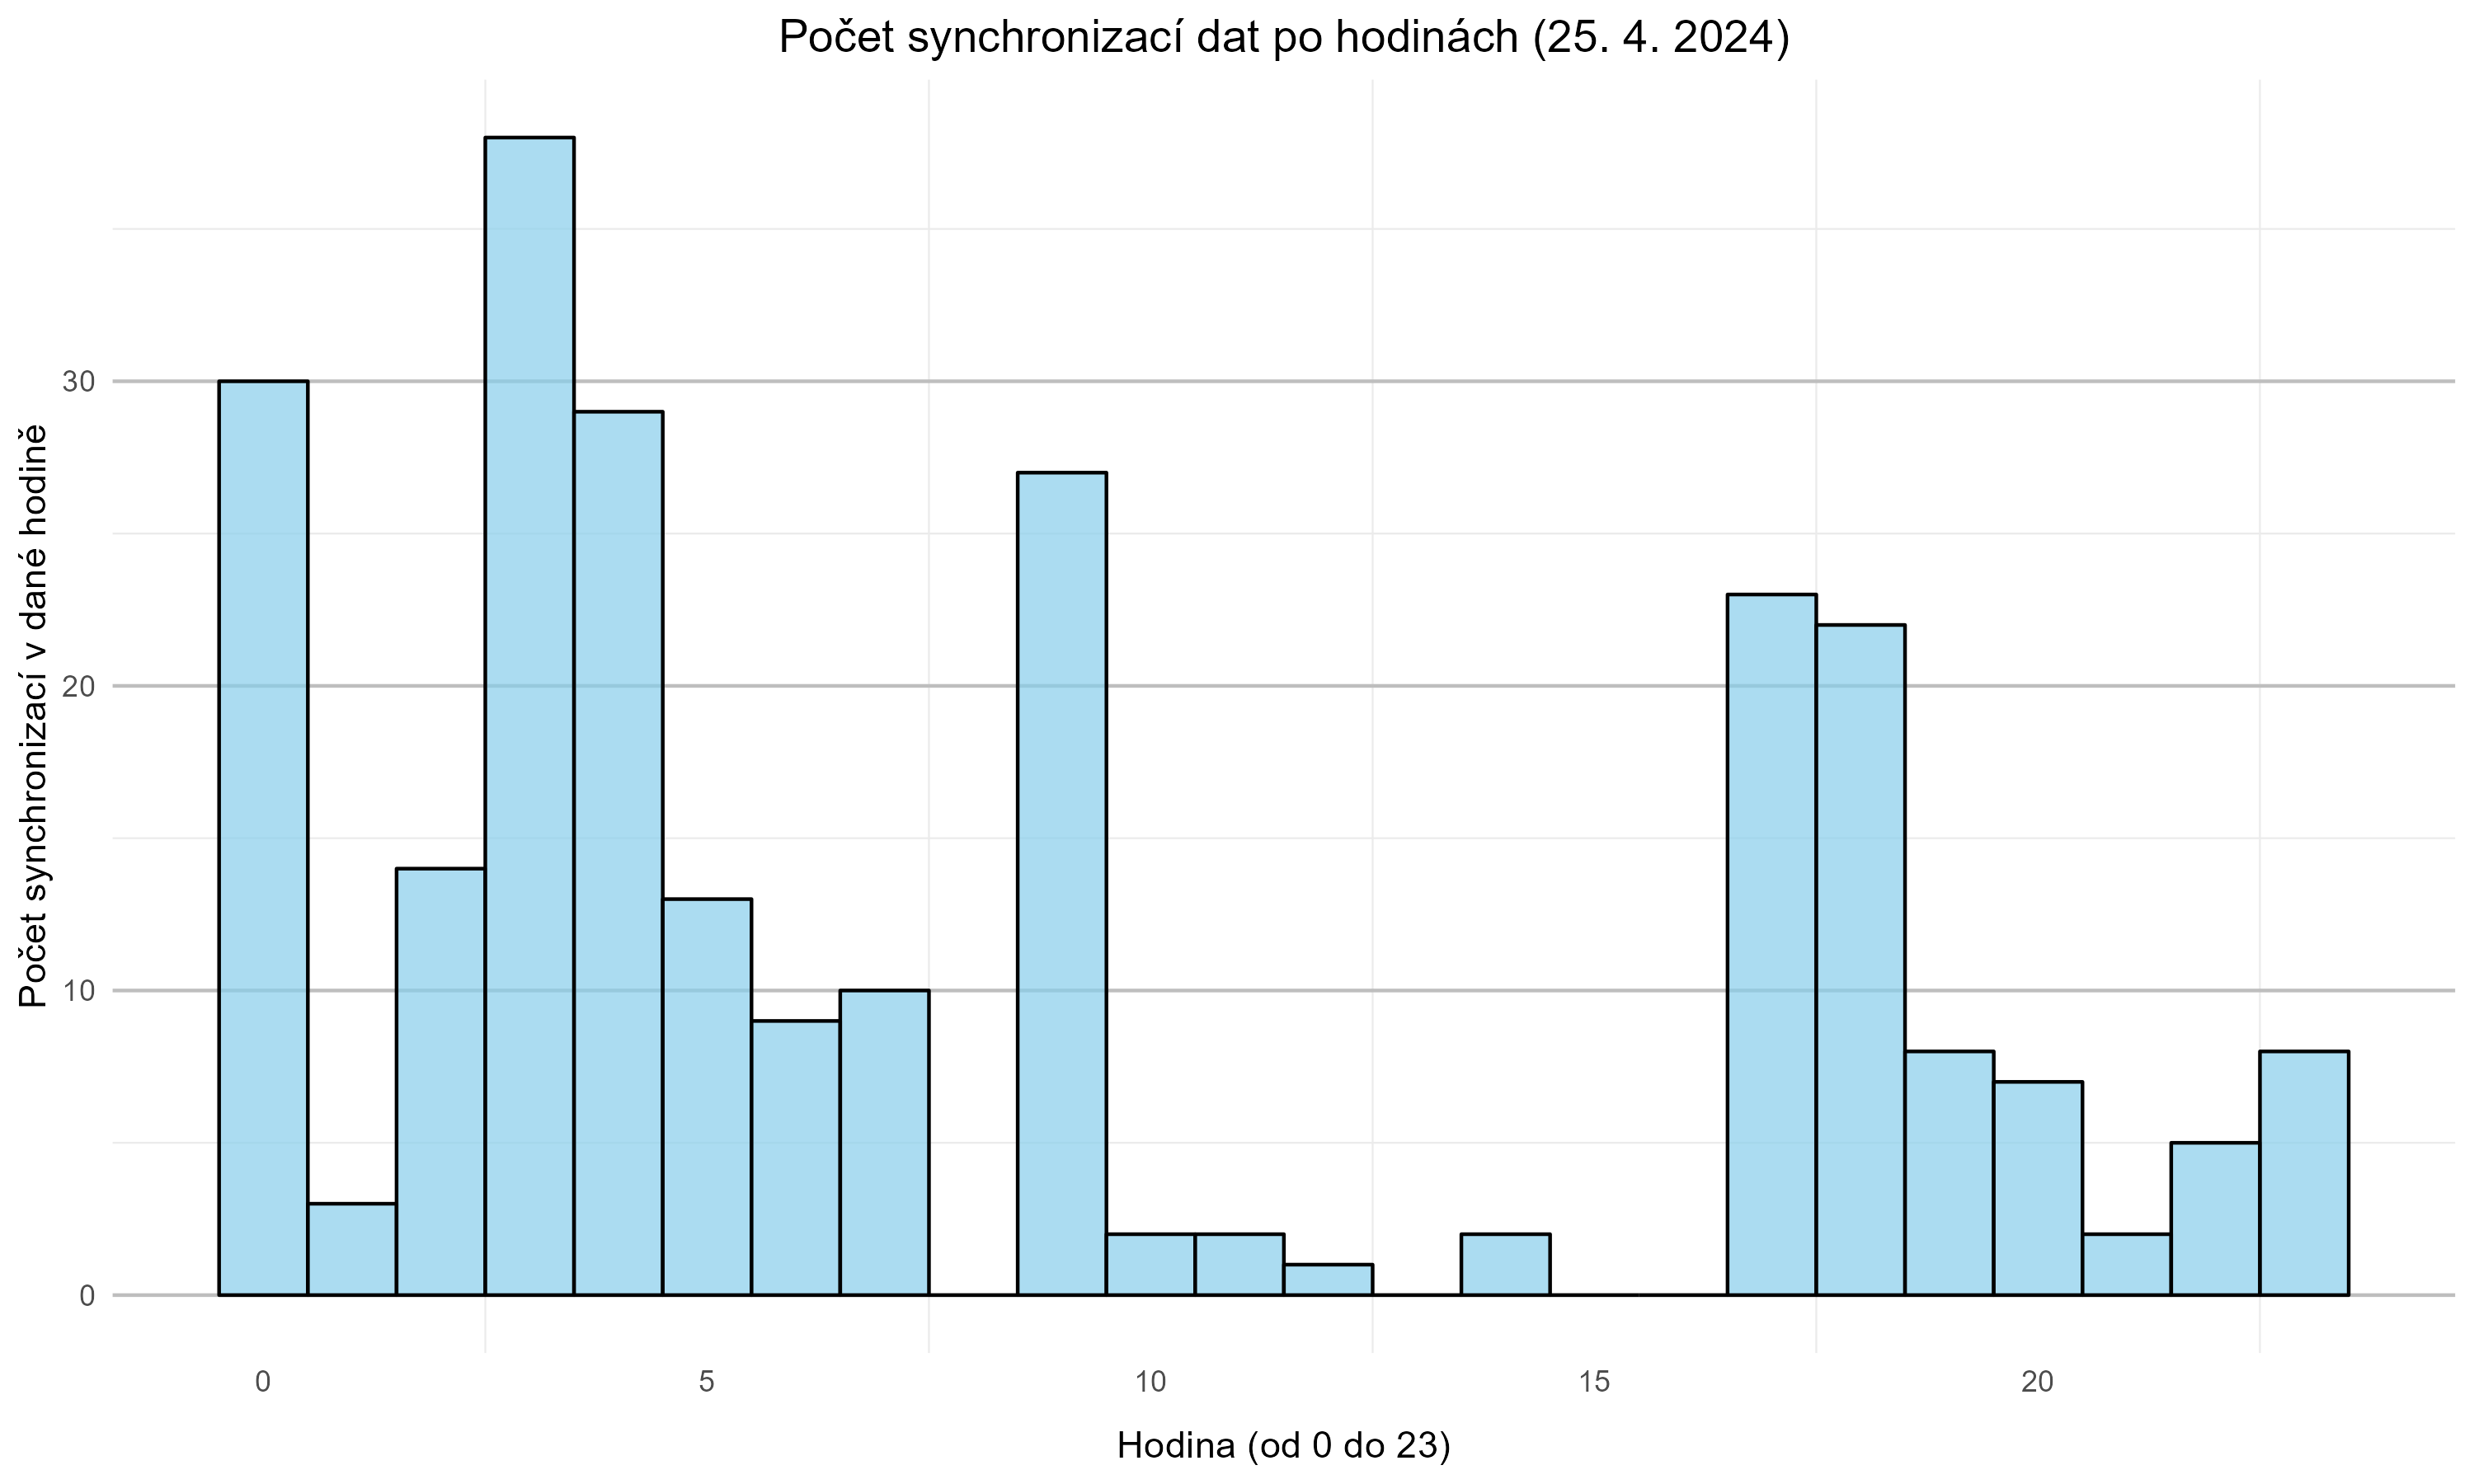
\includegraphics[width=12cm]{images/synchro_histogram.png}
	\caption{Histogram počtu synchronizací}
\end{figure}

\section{Testování GNSS modulu}

\subsubsection{Prvotní synchronizace}
Bylo zjištěno, že prvotní synchronizace bývá za vhodných podmínek (v~exteriéru nebo u~okna) provedena během několika sekund.

\subsubsection{Průběžná synchronizace}
Po prvotní synchronizaci získává modul čas nepřetržitě, pokud nedojde k~přerušení příjmu signálu (stínění antény).

\section{Testování NTP serveru}
Čas z~\zk{NTP} serveru bývá získán prakticky okamžitě a pokud nedojde k~přerušení internetového připojení získává zařízení čas nepřetržitě.

\section{Porovnání získaných časů}
Pro porovnání časů získaných z~NTP serveru, přijímače signálu DCF77 a GNSS přijímače byl vytvořen testovací kód pro Arduino UNO R4. Tento kód synchronizuje čas pomocí všech tří zmíněných metod a provádí záznam času každou minutu od spuštění Arduina.

\begin{table}[H]
    \centering
    \caption{Porovnání časů z~různých zdrojů}
    \begin{tabular}{|c|c|c|c|}
    \hline
    Arduino čas & NTP & DCF77 & GNSS \\
    \hline\hline
    00:04:00.00 & 10:27:12.52 & 10:27:12.55 & 10:27:12.68 \\ \hline
    00:05:00.00 & 10:28:12.50 & 10:28:12.55 & 10:28:12.65 \\ \hline
    00:06:00.00 & 10:29:12.49 & 10:29:12.55 & 10:29:12.64 \\ \hline
    00:07:00.00 & 10:30:12.49 & 10:30:12.54 & 10:30:12.69 \\ \hline
    00:08:00.00 & 10:31:12.48 & 10:31:12.54 & 10:31:12.62 \\ \hline
    \end{tabular}\\
\end{table}

Z~měřených dat je vidět, že získané časy se od sebe liší na úrovni setin až \text{desetin} sekundy. Tyto rozdíly mohou být způsobeny tím, že každý zdroj má lehce rozdílnou přesnost. \text{Nejvíce} se liší čas získaný pomocí GNSS přijímače, to může být způsobeno tím, že zpracování NMEA zprávy není dostatečně rychlé a dochází tedy ke zpoždění v~určení času. Pokud se chyba v~určení času pohybuje na úrovni pod jednu \text{desetinu} sekundy, lze očekávat, že chyba výsledného astronomického azimutu Slunce, způsobená určením času, bude mít velikost menší než 5\(^{cc}\).